%%%%%%%%%%%%%%%%%%%%%%%%%%%%%%%%%%%%%%%%%
% Beamer Presentation
% LaTeX Template
% Version 1.0 (10/11/12)
%
% This template has been downloaded from:
% http://www.LaTeXTemplates.com
%
% License:
% CC BY-NC-SA 3.0 (http://creativecommons.org/licenses/by-nc-sa/3.0/)
%
%%%%%%%%%%%%%%%%%%%%%%%%%%%%%%%%%%%%%%%%%

%----------------------------------------------------------------------------------------
%	PACKAGES AND THEMES
%----------------------------------------------------------------------------------------

\documentclass{beamer}

\mode<presentation> {

% The Beamer class comes with a number of default slide themes
% which change the colors and layouts of slides. Below this is a list
% of all the themes, uncomment each in turn to see what they look like.

%\usetheme{default}
%\usetheme{AnnArbor}
%\usetheme{Antibes}
%\usetheme{Bergen}
%\usetheme{Berkeley}
%\usetheme{Berlin}
%\usetheme{Boadilla}
%\usetheme{CambridgeUS}
%\usetheme{Copenhagen}
%\usetheme{Darmstadt}
%\usetheme{Dresden}
%\usetheme{Frankfurt}
%\usetheme{Goettingen}
%\usetheme{Hannover}
%\usetheme{Ilmenau}
%\usetheme{JuanLesPins}
%\usetheme{Luebeck}
\usetheme{Madrid}
%\usetheme{Malmoe}
%\usetheme{Marburg}
%\usetheme{Montpellier}
%\usetheme{PaloAlto}
%\usetheme{Pittsburgh}
%\usetheme{Rochester}
%\usetheme{Singapore}
%\usetheme{Szeged}
%\usetheme{Warsaw}

% As well as themes, the Beamer class has a number of color themes
% for any slide theme. Uncomment each of these in turn to see how it
% changes the colors of your current slide theme.

%\usecolortheme{albatross}
%\usecolortheme{beaver}
%\usecolortheme{beetle}
%\usecolortheme{crane}
%\usecolortheme{dolphin}
%\usecolortheme{dove}
%\usecolortheme{fly}
%\usecolortheme{lily}
%\usecolortheme{orchid}
%\usecolortheme{rose}
%\usecolortheme{seagull}
%\usecolortheme{seahorse}
%\usecolortheme{whale}
%\usecolortheme{wolverine}

%\setbeamertemplate{footline} % To remove the footer line in all slides uncomment this line
%\setbeamertemplate{footline}[page number] % To replace the footer line in all slides with a simple slide count uncomment this line

%\setbeamertemplate{navigation symbols}{} % To remove the navigation symbols from the bottom of all slides uncomment this line
}

\usepackage{graphicx} % Allows including images
\usepackage{booktabs} % Allows the use of \toprule, \midrule and \bottomrule in tables

%----------------------------------------------------------------------------------------
%	TITLE PAGE
%----------------------------------------------------------------------------------------

\title[Comparison of machine learning methods for stock return series]{Comparison of machine learning methods for stock return series} % The short title appears at the bottom of every slide, the full title is only on the title page
\author{Jian Wang } % Your name
\institute[Florida state university ] % Your institution as it will appear on the bottom of every slide, may be shorthand to save space
{Financial math Ph.D. candidate\\
\vspace{3ex}
Florida state university %%alifornia \\ % Your institution for the title page
\medskip
\textit{jwang@math.fsu.edu} % Your email address
}
\date{\today} % Date, can be changed to a custom date

\begin{document}

\begin{frame}
\titlepage % Print the title page as the first slide
\end{frame}

\begin{frame}
\frametitle{Overview} % Table of contents slide, comment this block out to remove it
\tableofcontents % Throughout your presentation, if you choose to use \section{} and \subsection{} commands, these will automatically be printed on this slide as an overview of your presentation
\end{frame}

%----------------------------------------------------------------------------------------
%	PRESENTATION SLIDES
%----------------------------------------------------------------------------------------

%------------------------------------------------
\section{Introduction} % Sections can be created in order to organize your presentation into discrete blocks, all sections and subsections are automatically printed in the table of contents as an overview of the talk
%------------------------------------------------

%\subsection{Subsection Example} % A subsection can be created just before a set of slides with a common theme to further break down your presentation into chunks

\begin{frame}
\frametitle{Introduction}
\begin{itemize}
\item \textbf{[Machine Learning:]} Machine learning is a method of teaching computers to make predictions based on historical data.  It is one important branch of artificial intelligence research area. Nowadays, those popular algorithms have been widely used in our financial engineering research area, for example, prediction of stock trend,  deal with big data problem such as limit order book problem.
\item \textbf{[Goal:]} In our research, we try to deal with the following tasks: \textbf{First}, combine Bayesian network and graphical lasso algorithm to deal with the high dimensional problem. \textbf{Second}, compare the efficiency of machine learning packages of language R and python. \textbf{Finally}, use machine learning methods to deal with the real world stock return data and try to predict the stock return series via those machine learning methods.  \\
\end{itemize}


\end{frame}

\section{DataSet}
\begin{frame}
\frametitle{Dataset}
The dataset is named stockdata which from huge package in R. It contained data that were
originally obtained from Yahoo! Finance. There are 1,258
observations representing 1,258 sequential trading days(form Jan 1 2003 to Jan 1 2008) and 452
variables, each of which was the day's closing price for a different
stock within the Standard \& Poor's 500.We also added two index into the data set, one is S\&P 500 and another is Nasdaq(so totally 454 variables).\\
Among all the stock data , we used Goldman Sachs stock return
series as our response variable and other stocks as the predictors to analyze the stock return series movement.
\begin{columns}
\column{2.3in}
\textbf{Company:}:
 \begin{figure}
     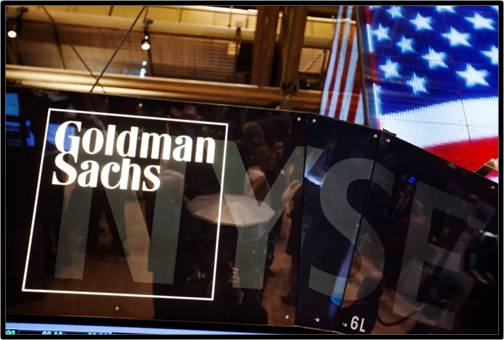
\includegraphics[width=0.6\textwidth, height=0.25\textheight]{gschart.jpg}
\end{figure}

\column{2.3in}

\textbf{Price:}:
\begin{figure}
     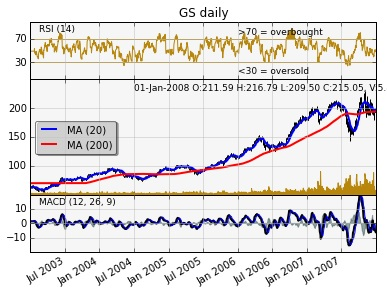
\includegraphics[width=0.6\textwidth, height=0.3\textheight]{gs_plot.jpg}
\end{figure}

\end{columns}
\end{frame}

\section{Methodology}
\begin{frame}
\frametitle{Methodology}
\textbf{Bayesian network} is a probabilistic graphical model (a type of statistical model)
that represents a set of random variables and their conditional dependencies via a directed acyclic graph (DAG)\\
The following chart is an example of BN:\\
 \begin{figure}
     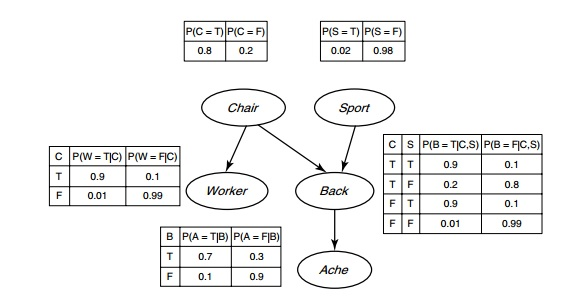
\includegraphics[width=0.9\textwidth]{bayesian.jpg}

    \end{figure}

\end{frame}

\begin{frame}

\frametitle{Methodology}
Our main concern is on the structure learning process since the structure learning process is exponentially increasing complicated and is the most challenging part in Bayesian network research area. The standard that we used to choose the optimal structure is the score based method.\\
\vspace{2ex}
BIC score:$BIC=-2*ln\hat{L}+K*ln(n)$, where:\\
\vspace{2ex}
$\hat{L}=$ maximum likelihood estimator, $k$ is the number of free parameters and $n$ is the number of observations, ie, the sample size.
 \begin{figure}
     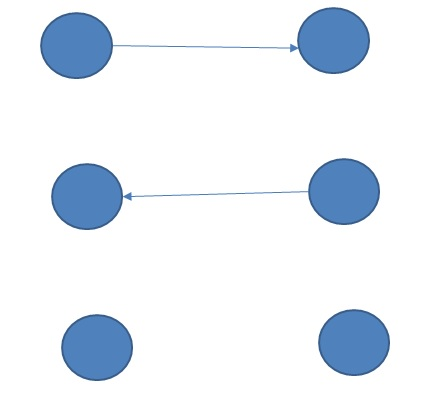
\includegraphics[width=0.4\textwidth, height=0.4\textheight]{learning.jpg}

    \end{figure}
\end{frame}

\begin{frame}
\frametitle{Methodology}
%
%\setbeamercovered{transparent}
%\begin{block}{Stock Return series}
%\begin{equation}
%R_t = ln( S_{t+1})-ln(S_t)
%\end{equation}
%Where $R_t$ is the stock return at trading day t and $S_t$ is the closing price of stock at trading day t.
%\end{block}
%\setbeamercovered{transparent}
\begin{block}{Linear regression}
\begin{equation}
\hat{\beta}^{ls}=argmin_{\beta}\{\sum_{i=1}^p{(y_i-\hat{y_i})^2}\}
\end{equation}
\end{block}
\begin{block}{Ridge regression}
\begin{equation}
\hat{\beta}^{ridge}=argmin_{\beta}\{\sum_{i=1}^p{(y_i-\hat{y_i})^2}+{\color{red}\lambda \sum_{j=1}^p\beta_j^2}\}
\end{equation}
\end{block}

\begin{block}{Lasso regression}
\begin{equation}
\hat{\beta}^{lasso}=argmin_{\beta}\{\sum_{i=1}^p{(y_i-\hat{y_i})^2}+{\color{red}\lambda\sum_{j=1}^p |\beta_j|}\}
\end{equation}
\end{block}

\end{frame}


\begin{frame}
\frametitle{Methodology}
Comparison of L1 and L2 Penalized Model \\
\begin{columns}
\column{2.3in}
	\begin{block}{Ridge regression}
$\hat{\beta}^{ridge}=argmin_{\beta}\{\sum_{i=1}^p{(y_i-\hat{y_i})^2}+{\color{red}\lambda \sum_{j=1}^p\beta_j^2}\}$

\end{block}
\textbf{Coefficients}:
 \begin{figure}
     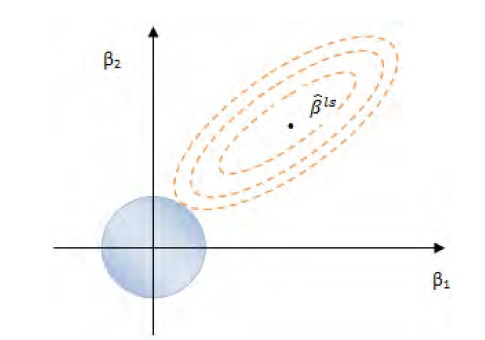
\includegraphics[width=0.9\textwidth, height=0.5\textheight]{ridge.jpg}

    \end{figure}

\column{2.3in}
\begin{block}{Lasso regression}

$\hat{\beta}^{lasso}=argmin_{\beta}\{\sum_{i=1}^p{(y_i-\hat{y_i})^2}+{\color{red}\lambda\sum_{j=1}^p |\beta_j|}\}$

\end{block}

\textbf{Coefficients}:
 \begin{figure}
     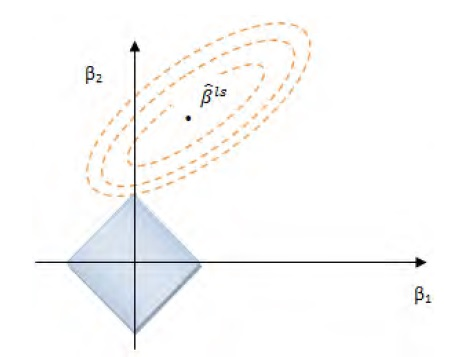
\includegraphics[width=0.9\textwidth, height=0.5\textheight]{lasso.jpg}

    \end{figure}
\end{columns}


\end{frame}

\begin{frame}
\frametitle{Methodology}
Comparison of L1 and L2 Penalized Model \\
\begin{columns}
\column{2.3in}
	\begin{block}{Ridge regression}
$\hat{\beta}^{ridge}=argmin_{\beta}\{\sum_{i=1}^p{(y_i-\hat{y_i})^2}+{\color{red}\lambda \sum_{j=1}^p\beta_j^2}\}$

\end{block}
\textbf{Path:}:
 \begin{figure}
     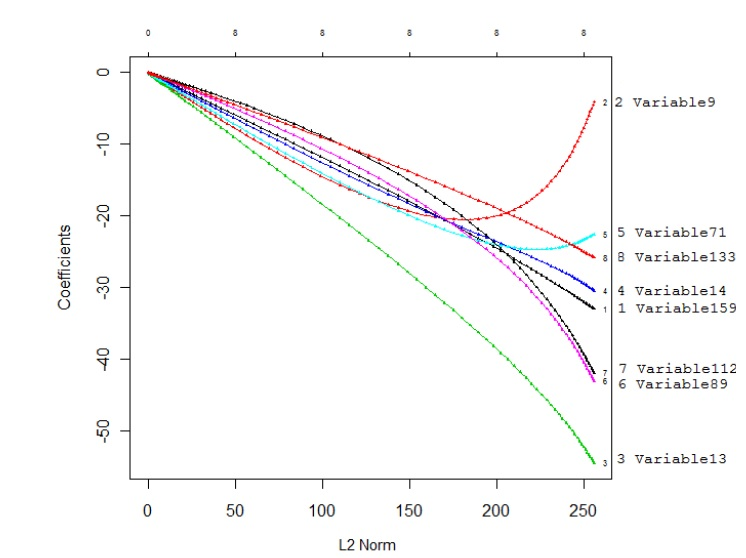
\includegraphics[width=0.9\textwidth, height=0.5\textheight]{ridge_p.jpg}

    \end{figure}

\column{2.3in}

\begin{block}{Lasso regression}

$\hat{\beta}^{lasso}=argmin_{\beta}\{\sum_{i=1}^p{(y_i-\hat{y_i})^2}+{\color{red}\lambda\sum_{j=1}^p |\beta_j|}\}$

\end{block}

\textbf{Path:}:
 \begin{figure}
     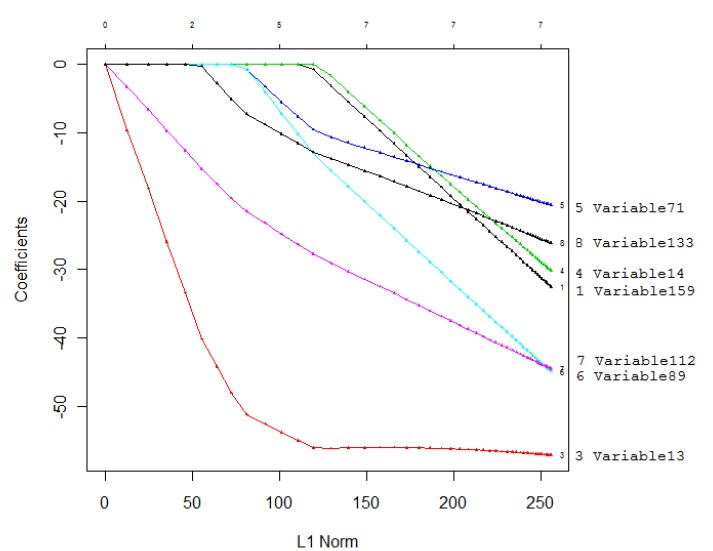
\includegraphics[width=0.9\textwidth, height=0.5\textheight]{lasso_p.jpg}

    \end{figure}
\end{columns}

\end{frame}

\begin{frame}
\frametitle{Methodology}
  \setbeamercovered{transparent}
  \begin{block}{Glasso:}
    Suppose we have N multivariate normal observations of dimension p , with mean $\mu$ and covariacne $\Sigma$. Let $\Theta=\Sigma^{-1}$ and $S$ be the empirical covariance matrix, the problem is to maximize the log- likelihood \\
    \begin{center}
    $lnP(X|u,\Sigma)=-\frac{N}{2}ln|\Sigma|-\frac{1}{2}\sum(x_n-u)^T \Sigma^{-1}(x_n-u)$\\
    combined with the $L_1$ penalty\\
    $ln |\Theta|- tr(S\Theta))-\lambda||\Theta||_1$
  \end{center}
  \end{block}

  \begin{block}<2>{Algorithm}
  Many algorithms for this problem, The following might be the oldest and simple one by Meinshausen and Buhlmann(2006)
    \begin{itemize}
        \item  Estimate a sparse graphical model by fitting a lasso model to each variable, using others as predictors
        \item  Set $\Sigma_{ij}^{-1}$ to be non zero, if either the estimated coefficient of variable i on j, or the
        estimated coefficient of variable j on i, is non-zero
    \end{itemize}
  \end{block}
\end{frame}

\begin{frame}
\frametitle{Bayesian-Glasso model}
 For the high dimensional problem, it is not very easy to built the Bayesian network due to its exponentially increasing complexity. \\
 Our idea is to first use the Glasso model to conduct the model selection and then use Bayesian network structure learning process
 to define the network structure. \\
   \setbeamercovered{transparent}
   \begin{block}<2>{Algorithm}
    \begin{itemize}
        \item  Use Glasso algorithm to find the edges among variables
        \item  Use greedy search methods to change the direction only on those existed edges
        \item  Choose the direction which has the optimal BIC score
        \item  Finish when all the edges are reached or attain the maximum iteration numbers
    \end{itemize}
  \end{block}

\end{frame}


\begin{frame}
\frametitle{Methodology}
\setbeamercovered{transparent}
\begin{block}{Logistic Regression}
\begin{equation}
ln{\frac{F(x)}{1-F(x)}}=\beta_0+\sum_i\beta_ix_i
\end{equation}
\end{block}
\begin{block}{Support vector machine}
\begin{columns}
\column{2.6in}
\scriptsize {
Try to maximize the margin: $r=1/||w||,y_j=1,-1$\\
Primal form:\\
$\max\limits_{W,b}\ r= 1/||W||$\\
$s.t.(W^Tx_j+b)y_j>=1$\\
Dual form:\\
$\max\limits_{\alpha_1,...,\alpha_M}\ \sum\alpha_l-\frac{1}{2}\sum_{j=1}^{M}\sum_{k=1}^{M}\alpha_j\alpha_k y_j y_k<X_j,X_k>$\\
s.t.$\alpha_l\geq 0$, $\sum_{l=1}^{M}\alpha_ly_l=0$
}
\column{2in}
\begin{figure}
     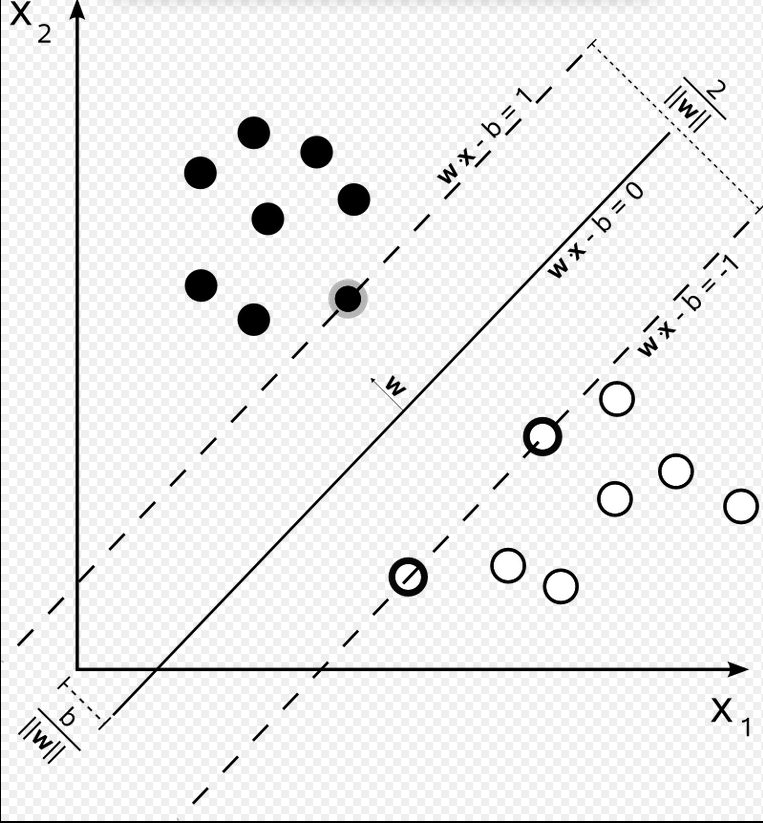
\includegraphics[width=0.6\textwidth, height=0.35\textheight]{svm.png}
\end{figure}
\end{columns}
\end{block}
\end{frame}


\begin{frame}
\frametitle{Methodology}
\setbeamercovered{transparent}
\begin{block}{Higher dimensional situations}
sometimes, in lower dimension we can not separate the data properly, so we need to project the data to the high dimensions\\
\end{block}
\begin{block}{Examples}
\begin{columns}
\column{2.3in}
\begin{figure}
     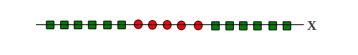
\includegraphics[width=0.5\textwidth, height=0.1\textheight]{1d.png}
\end{figure}
\begin{figure}
     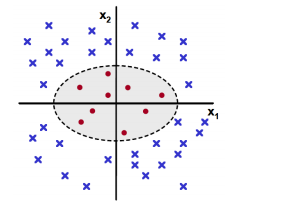
\includegraphics[width=0.5\textwidth, height=0.3\textheight]{2d.png}
\end{figure}

\column{2.3in}
\begin{figure}
     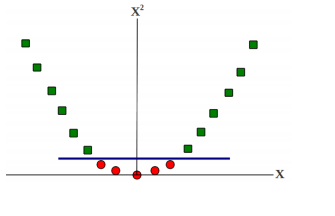
\includegraphics[width=0.5\textwidth, height=0.2\textheight]{1d_2.png}
\end{figure}
\begin{figure}
     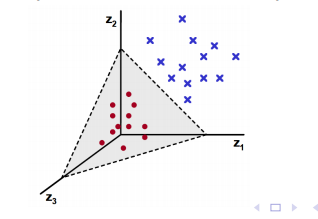
\includegraphics[width=0.5\textwidth, height=0.2\textheight]{2d_2.png}
\end{figure}
\end{columns}
\end{block}
\end{frame}


\begin{frame}
\frametitle{Methodology}
\setbeamercovered{transparent}
\begin{block}{Kernel functions}
We can use the kernel function to calculate the inner product in high dimensional cases in its original feature spaces.
\end{block}
\begin{block}{Example}
$k(x,z)=(x^Tz)^2$\\
$=(x_1z_1+x_2z_2)^2$\\
$=x_1^2z_1^2+x_2^2 z_2^2+2x_1x_2z_1z_2$\\
$=(x_1^2,\sqrt{2}x_1x_2,x_2^2)^T(z_1^2,\sqrt{2}z_1z_2,z_2^2)$\\
$=\Phi(x)^T\Phi(z)$\\
\end{block}
\begin{block}{Kernel functions that we used}
\begin{itemize}
        \item  Linear kernel\\
        \item  Polynomial Kernel\\
        \item  Radial basis function kernel\\
    \end{itemize}

\end{block}

\end{frame}

\begin{frame}
\frametitle{Methodology }
  \setbeamercovered{transparent}
  \begin{block}{Reference}
   \begin{itemize}
        \item  Tibshirani, R. (1996). "Regression shrinkage and selection via the lasso". Journal of the Royal Statistical Society, Series B 58 (1): 267–288. JSTOR 2346178
        \item Hoerl, A.E. and Kennard, R. (1970). Ridge regression: Biased
estimation for nonorthogonal problems. Technometrics, 12:
55-67
        \item Vapnik, V. (1995). "Support-vector networks". Machine Learning 20 (3): 273. doi:10.1007/BF00994018
    \end{itemize}
  \end{block}

  \begin{block}<2>{Packages}
    \begin{itemize}
        \item  R packages: glm, glmnet, e1071,bnlearn,huge
        \item  Python packages: sklearn (svm, ridge, lasso, logistic)
    \end{itemize}
  \end{block}

\end{frame}


\section{Numerical results}

\begin{frame}
\frametitle{Numerical results}
\begin{itemize}
        \item  Same day stock return series analysis:\\
        we use the same day stock return series to build the machine learning models. For the Bayesian network, we only use the R package. For the  logistic regression, ridge regression, lasso and svm, we used different languages(R and Python) and also compare the CPU time.
        To test the accuracy rate of model, we choose the first 1000 data as training data and the last remaining 257 data as testing. GS as response(discretized as 1 and -1) and the other 453 stocks as predictors.\\
        \item  Predict the stock data:\\
        we used the last one day, two day,... to last five day stock returns as the predictors and today's GS return series as response to see if our model can be used to predict the stockdata.\\
        Still use the first 1000 data as training and the remaining 252 data as testing. GS as the response and the other 2270 variables as predictors.\\
    \end{itemize}

\end{frame}

\begin{frame}
\frametitle{Numerical results}
\begin{block}{Bayesian network}
\begin{table}[h!]\small
  \caption{10 companies}
\begin{center}
    \begin{tabular}{| c | c| c | }
    \hline
    Stock code& Industry & Company name\\
    \hline
GS&Financials&Goldman Sachs Group\\
JPM&Financials&JPMorgan Chase \& Co.\\
MSFT&Information Technology&Microsoft Corp.\\
IBM&Information Technology&International Bus. Machines\\
T&Telecommunications Services&AT\&T Inc\\
VZ&Telecommunications Services&Verizon Communications\\
WMT&Consumer Staples&Wal-Mart Stores\\
KO&Consumer Staples&Coca Cola Co.\\
AMZN&Consumer Discretionary&Amazon.com Inc\\
BBY&Consumer Discretionary&Best Buy Co. Inc.\\

\hline
\end{tabular}
\end{center}
\end{table}
\end{block}

\end{frame}
\begin{frame}
\frametitle{Numerical results}
\setbeamercovered{transparent}

\begin{block}{Results for simple cases}
\begin{columns}
\column{1.5in}
\begin{figure}
     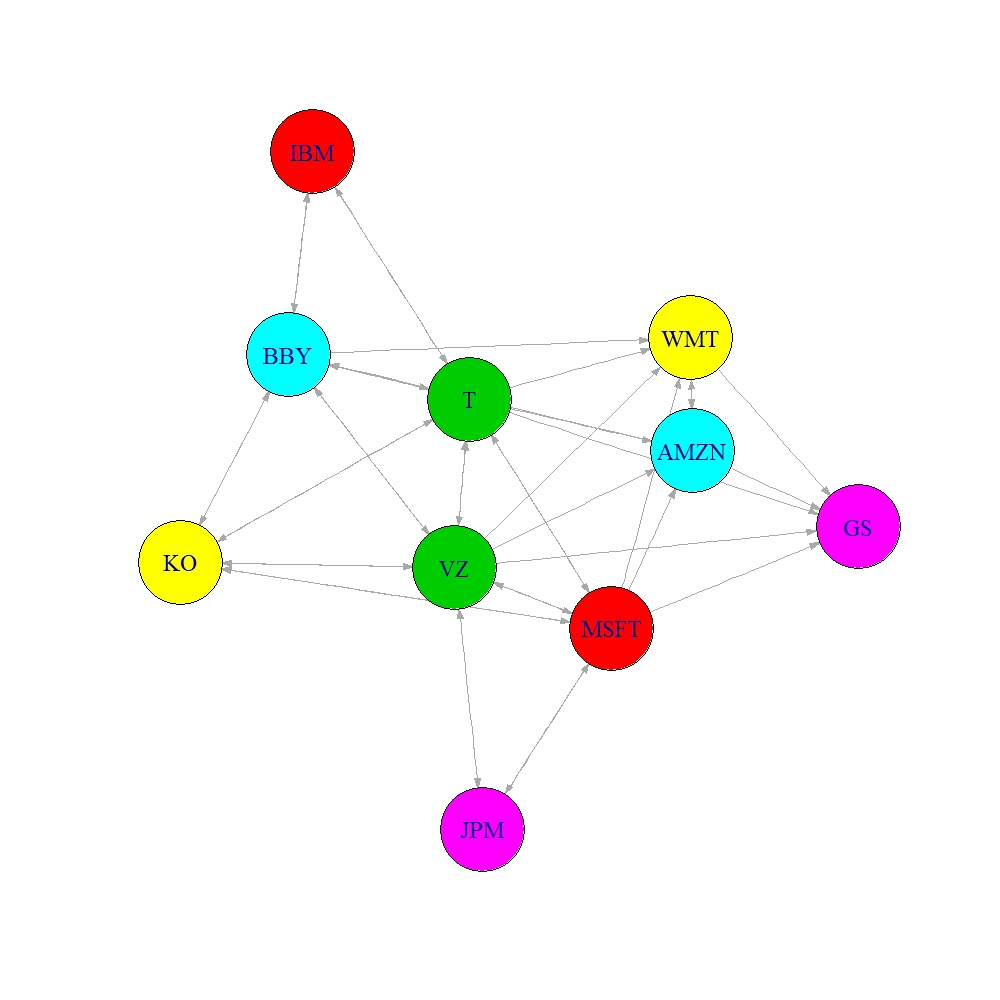
\includegraphics[width=1\textwidth, height=0.5\textheight]{10stocks.jpeg}
\end{figure}

\column{1.5in}
\begin{figure}
     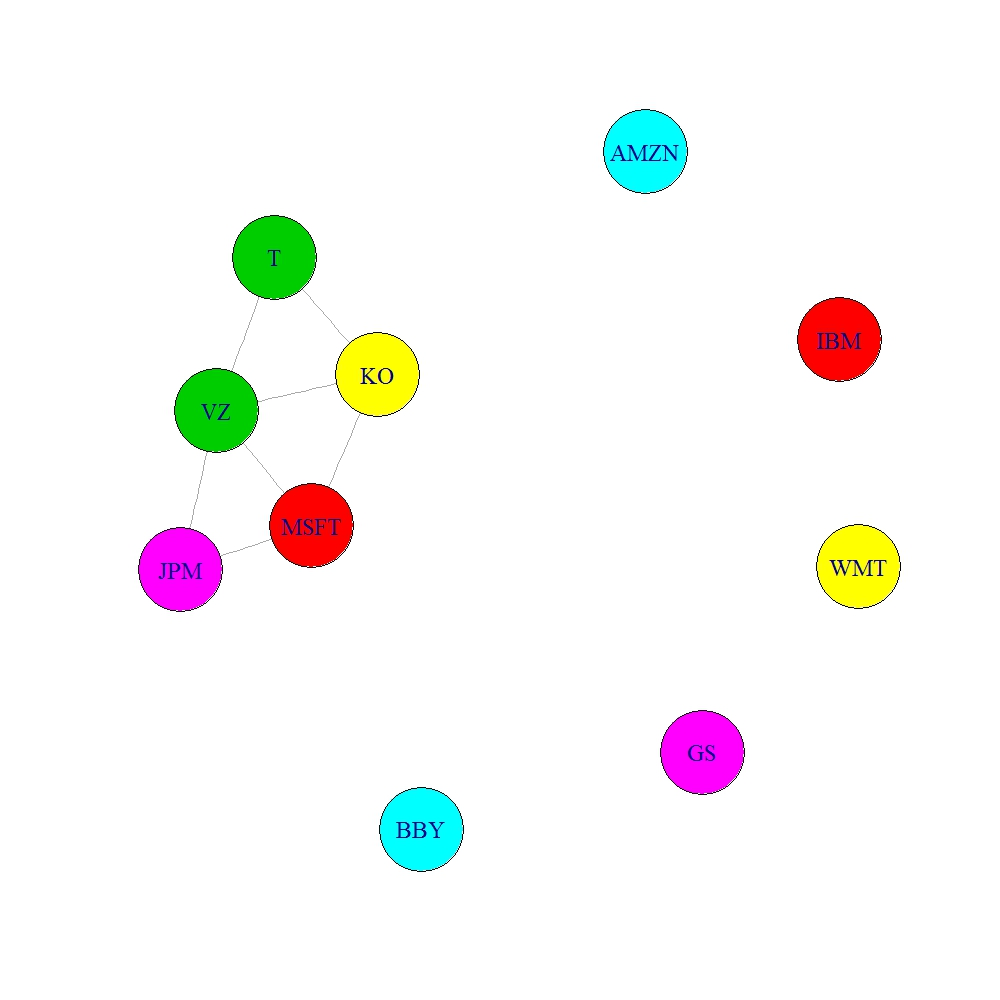
\includegraphics[width=1\textwidth, height=0.5\textheight]{10stocks_huge.jpeg}
\end{figure}
\column{1.5in}
\begin{figure}
     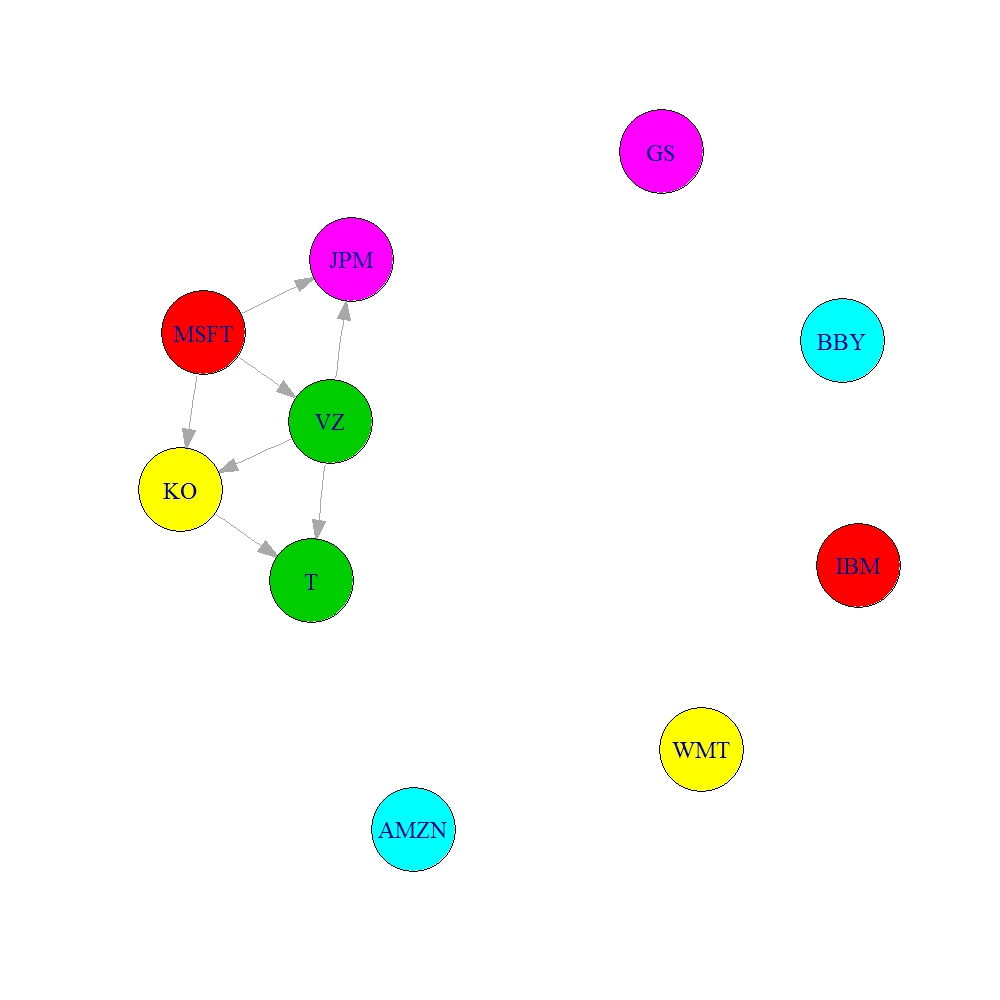
\includegraphics[width=1\textwidth, height=0.5\textheight]{10stocks_bn_glasso.jpeg}
\end{figure}
\end{columns}
\end{block}
\end{frame}

\begin{frame}
\frametitle{Numerical results}
\setbeamercovered{transparent}
\begin{block}{Results for total stocks}
     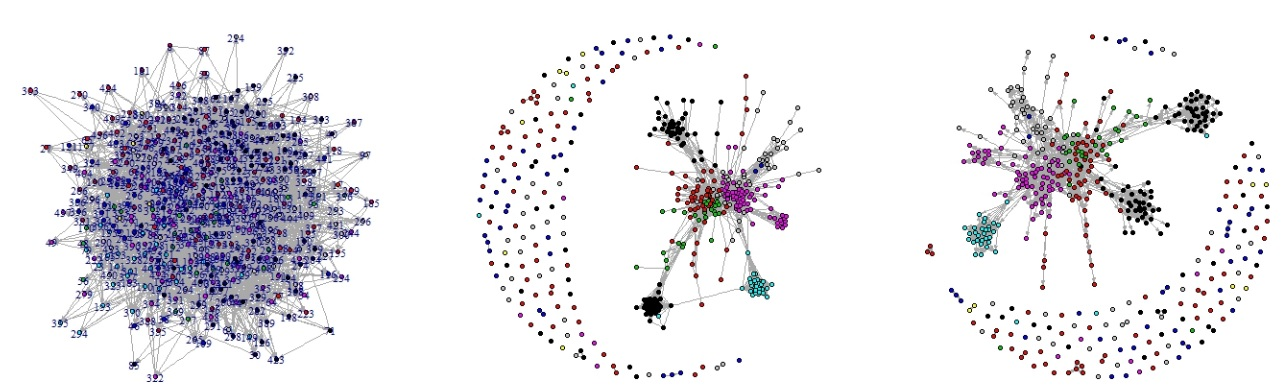
\includegraphics[width=0.9\textwidth, height=0.4\textheight]{stock.jpg}
\end{block}
\end{frame}

\begin{frame}
\frametitle{Numerical results}
\begin{columns}
\column{2.3in}
	\begin{block}{CPU Time for R}
We changed the number of samples from 50 to 800, doubled each time to test the running time for the different machine learning methods:\\
\begin{figure}
     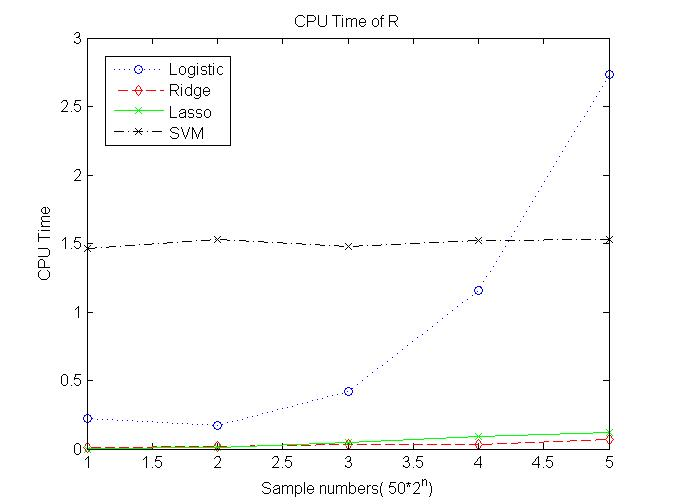
\includegraphics[width=0.8\textwidth, height=0.5\textheight]{cputime_r.jpg}

    \end{figure}

\end{block}

\column{2.3in}
\begin{block}{CPU Time for Python}
We changed the number of samples from 50 to 800, doubled each time to test the running time for the different machine learning methods:\\
\begin{figure}
     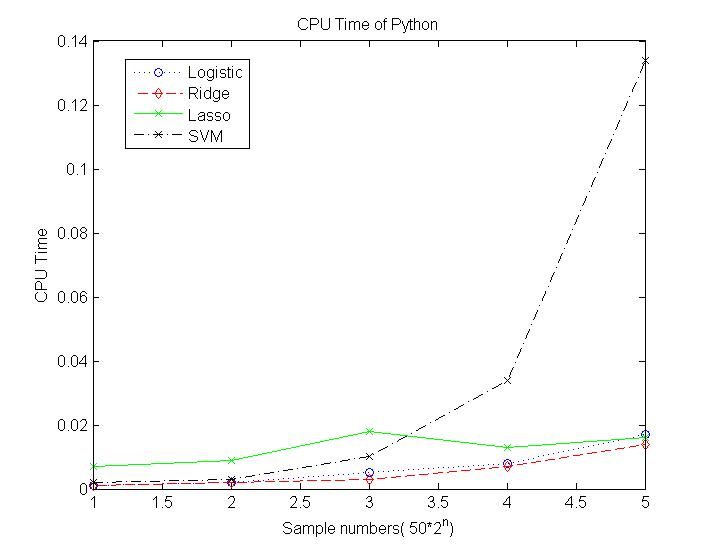
\includegraphics[width=0.8\textwidth, height=0.5\textheight]{cputime_python.jpg}

    \end{figure}
\end{block}

\end{columns}

\begin{block}{Results:}
Logistic and svm methods took long time than the other two in R , svm and lasso took long time in python.\\

\end{block}


\end{frame}

\begin{frame}
\frametitle{Numerical results}
\begin{block}{Comparison of CPU time for python and R }
\begin{center}
 \begin{figure}
     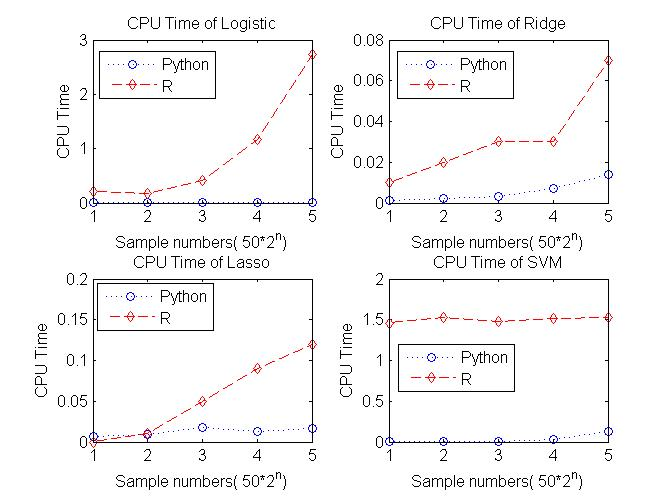
\includegraphics[width=0.8\textwidth, height=0.7\textheight]{cputime_python_r.jpg}

    \end{figure}
\end{center}
\end{block}

\begin{block}{Results:}
Python took smaller time for all the four methods compared with R.
\end{block}

\end{frame}

\begin{frame}
\frametitle{Numerical results:}

\begin{block}{Accuracy rate:}
\begin{table}[h!]\large
  \caption{Accuracy rate}
\begin{center}
    \begin{tabular}{| c | c| c | }
    \hline
    Methods& Python &  R\\
    \hline
Logistic  &69.8\%&	68.4\%\\
Ridge($\lambda$=1)&73.9\%	&77.4\%\\
Lasso($\lambda$=0.01)&78.6\%&	79.0\%\\
svm(linear)&72.4\%	&71.8\%\\
svm(poly)&74.3\%&	71.2\%\\
svm(rbf)&75.1\%	&72.8\%\\
\hline
\end{tabular}
\end{center}
\end{table}
\end{block}

\begin{block}{Results:}
\begin{itemize}
        \item lasso ($\lambda$=0.01) and svm (rbf) performed good for both two languages. 
        \item Python performed better in most cases but the difference is not significant.
    \end{itemize}

\end{block}
\end{frame}


\begin{frame}
\frametitle{Numerical results:}
\begin{block}{Predicted}
\begin{equation}
R_t^{GS} = \sum_{i=1:5}{\sum_{j=1:454}\beta_{i,j}R_{t-i}^j}
\end{equation}
\end{block}

\begin{block}{Predict:}
\begin{table}[h!]\large
  \caption{Accuracy rate and CPU time}
\begin{center}
    \begin{tabular}{| c | c|c|}
    \hline
    Methods& Accuracy rate& CPU time \\
    \hline
Logistic  &51.2\%&0.1210\\
Ridge($\lambda$=1)&54.0\%&0.1230\\
Lasso($\lambda$=0.01)&49.2\%&0.0940\\
svm(linear)&52.8\%&1.1931\\
svm(poly)&45.6\%&1.2800	\\
svm(rbf)&47.2\%&1.2921\\
Bayesian Glasso&51.6\%&around two hours\\
\hline
\end{tabular}
\end{center}
\end{table}
\end{block}
\end{frame}



\section{Future work}
\begin{frame}
\frametitle{Future work}
    \begin{itemize}
        \item  Compare with the time series model, such as Garch(machine learning methods can consider the whole economic environment while time series cannot)
        \item  Deal with the high frequency data instead of daily data
      \end{itemize}
\end{frame}

\section{Questions}
\begin{frame}
\frametitle{QA}
\begin{center}
\huge{Thanks a lot and Questions}
\end{center}
\end{frame}
%
%%------------------------------------------------------------------
%
\end{document} 